% -*- root: ../main.tex -*-
%!TEX root = ../main.tex
% this file is called up by main.tex
% content in this file will be fed into the main document
% vim:textwidth=80 fo=cqt

In   this    section,   the    quadratic   approximation   of    ionic   spatial
concentration,   that  underpins   the  electrolyte   model  in   many  improved
\gls{spm}  formulations  is  presented.  The  steps  involved  in  deriving  the
quadratic   approximation   is  detailed   in~\cref{subsec:quadraticmodelderiv}.
In~\cref{subsec:quadraticsimresultsanalysis},  an analysis  of  the weakness  of
this  model is  performed  based  on the  results  from  applying the  quadratic
approximation scheme. Mitigation of this critical drawback lead to this author's
decoupled  spatio-temporal electrolyte  concentration model  structure which  is
presented next in~\cref{sec:newelectrolytemodel}.

\subsection{Model derivation}\label{subsec:quadraticmodelderiv}

\begin{figure}[!htb]
    \captionsetup{singlelinecheck=off}
    \centering
    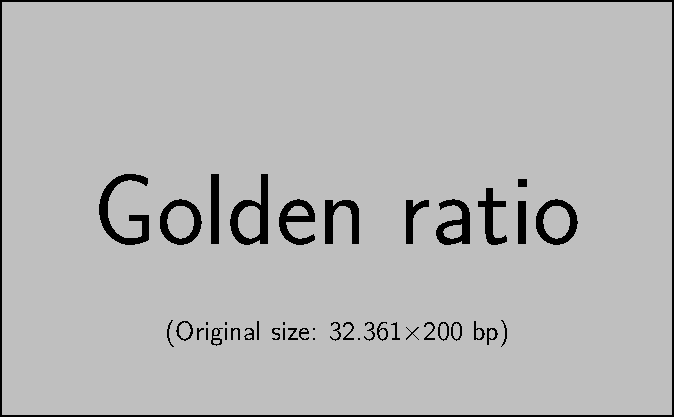
\includegraphics{placeholder_images/example-image-golden.pdf}
    \caption[Co-ordinate systems for quadratic approximation of
    electrolyte concentration]{Schematic diagram of the electrochemical sandwich
        consisting of
        \begin{enumerate*}[label=\itshape\alph*\upshape)]
            \item negative electrode,
            \item separator, and
            \item positive electrode
        \end{enumerate*} depicting the co-ordinate system used in deriving the
        quadratic approximation profile. The global spatial co-ordinate is $x
        \in \{0,l_\text{tot}\}$, where $l_\text{tot} = l_\text{neg} +
        l_\text{sep} + l_\text{pos}$. Local co-ordinate systems specific to each
        region are also defined. It should be noted that the positive
    electrode's local co-ordinate axis direction is reversed.}
    \label{fig:coordsquadapprox}
\end{figure}

The  schematic  in~\cref{fig:coordsquadapprox}  shows   the  definition  of  the
co-ordinate  systems  used  in  deriving the  polynomial  approximation  of  the
electrolyte concentration  profile. The globally defined  $x$ co-ordinate starts
at  the negative  current  collector  interface ($x=0$)  and  terminates at  the
positive  current  collector  interface  ($x =  l_\text{tot},\,  l_\text{tot}  =
l_\text{neg} +  l_\text{sep} +  l_\text{pos}$). Three local  co-ordinate systems
$z_\mu$  valid  only  within  their  respective regions  are  also  defined.  In
particular, it  must be  noted that  the direction  of the  local $z_\text{pos}$
co-ordinate axis is opposite to that of  the other two local co-ordinate axes as
well as the global co-ordinate axis. In subsequent usages, the suffix in $z_\mu$
is dropped and  the reader is advised  to infer the region of  validity from the
usage  context  which are  unambiguous  as  they  occur in  separate  equations.
Furthermore, the  notation of  the three regions  $\{\text{neg, sep,  pos}\}$ is
abbreviated  to $\{n,s,p\}$  respectively in  all mathematical  expressions. The
author  is convinced  that this  notation does  not detract  from following  the
derivations, but rather aids it by keeping the notations compact.

A  standard  quadratic expression  is  chosen  a  priori for  approximating  the
electrolyte concentration profile within each region.
\begin{alignat}{2}
    c_\ensub(z,t) & = a_2(t) z^2 + a_1(t) z + a_0(t) \qquad &  & 0 \le z \le l_\text{n}\label{eq:cenqquadstart}   \\
    c_\essub(z,t) & = a_5(t) z^2 + a_4(t) z + a_3(t) \qquad &  & 0 \le z \le l_\text{s}\label{eq:cesqquadstart}   \\
    c_\epsub(z,t) & = a_8(t) z^2 + a_7(t) z + a_6(t) \qquad &  & 0 \le z \le l_\text{p}\label{eq:cepqquadstart}
    \shortintertext{where     the    coefficient     vector    $\vec{a}(t)     =
        \vect{a_0(t),a_1(t),   \dots  ,a_8(t)}$   is  to   be  determined   at  each
        time-step\footnotemark.  Applying  boundary  conditions of  the  electrolyte
        diffusion equation from  the \gls{dfn} model~(refer~\cref{eq:dfnliquiddiff})
        to~\crefrange{eq:cenqquadstart}{eq:cepqquadstart},  it  is clear  that  $a_1
        =  0$ and  $a_7  = 0$.  Thus,~\crefrange{eq:cenqquadstart}{eq:cepqquadstart}
    become}
    c_\ensub      & = a_2 z^2 + a_0         \qquad          &  & 0 \le z \le l_\text{n}\label{eq:cenquadreduced} \\
    c_\essub      & = a_5 z^2 + a_4 z + a_3 \qquad          &  & 0 \le z \le l_\text{s}\label{eq:cesquadreduced} \\
    c_\epsub      & = a_8 z^2 + a_6         \qquad          &  & 0 \le z \le l_\text{p}\label{eq:cepquadreduced}
\end{alignat}
\footnotetext{In rest of  the equations, time-dependence of  the coefficients is
    dropped from  the notation. It is  implicitly noted that they  are time-varying.
    Similarly, spatio-temporal dependence of the electrolyte concentration functions
    $c_\text{e,j}$ is omitted  in circumstances where such explicit  notation is not
crucial  for  understanding.} with  the  coefficient  vector being  modified  to
$\vec{a} = \vect{a_0,a_2, \dots ,a_6, a_8}$.

% -*- root: ../main.tex -*-
%!TEX root = ../main.tex
% this file is called up by main.tex
% content in this file will be fed into the main document
% vim:nospell textwidth=180 foldlevelstart=3 foldlevel=3 conceallevel=0

\begin{table}[!htb]
    \centering
    \caption[Electrolyte equations \& boundary conditions of \glsfmtshort{dfn} model in separator]{Electrolyte-specific governing equations and boundary conditions of the \glsfmtlong{dfn} model within the separator domain.}
    \label{tbl:dfnelectrolyteeqnsinsep}
    \begingroup
    \makeatletter\def\f@size{9.25}\check@mathfonts
    \addtolength{\jot}{0.875em}
    \begin{tabular*}{\textwidth}{@{} l c r l r @{}}
        \toprule
        \multicolumn{1}{c}{\small Region} & \small Governing equations & \multicolumn{2}{c}{\small Boundary conditions } & {} \\
        {} & {} & \multicolumn{2}{c}{\scriptsize $(l_\text{neg} \coloneqq l_\text{n},\, l_\text{sep} \coloneqq l_\text{s},\, l_\text{pos} \coloneq l_\text{p})$} \\
        \midrule
        \multicolumn{1}{l |}{{\rotatebox[origin=c]{90}{\makecell{\footnotesize Separator\\ \scriptsize $\delta \in \{\text{sep}\}$}}}} &
        $\begin{aligned}
            \vphantom{D_{\text{\tiny eff}_\text{n}}\!\! \! \!\, \diffp{c_\text{e}}{x}{\mathrlap{x = l^{-}_\text{n}}}} \varepsilon_\delta \diffp{c_\text{e}}{t} &=D_\effdelta  \diffp[2]{c_\text{e}}{x} \\[-0.75em]
            \vphantom{D_{\text{\tiny eff}_\text{s}}\!\! \! \!\, \diffp{c_\text{e}}{x}{\mathrlap{x=(l_{\text{n}} + l_\text{s})^{-}}}}\\[1.25em]
            \vphantom{\kappa_{\text{\tiny eff}_\text{n}}\!\! \! \!\, \diffp{c_\text{e}}{x}{\mathrlap{x = l^{-}_\text{n}}}\hspace{5mm} =\kappa_{\text{\tiny eff}_\text{s}}\!\!\!\!\,\diffp{c_\text{e}}{x}{\mathrlap{x = l^{+}_\text{n}}}} \frac{I}{A} &= \overline{\kappa}_\effdelta \left( \diffp[2]{\phi_\text{e}}{x} + \frac{2 R T}{F} (t^0_{+}-1)\diffp[2]{ \ln c_\text{e}}{x}\right) \\[-0.75em]
            \vphantom{\kappa_{\text{\tiny eff}_\text{s}}\!\! \! \!\, \diffp{c_\text{e}}{x}{\mathrlap{x=(l_{\text{n}} + l_\text{s})^{-}}}} \\
        \end{aligned}$ &
        $\begin{aligned}
    \vphantom{D_{\text{\tiny eff}_\text{n}}\!\! \! \!\, \diffp{c_\text{e}}{x}{\mathrlap{x = l^{-}_\text{n}}}} \qquad c_\text{e}\Bigr\rvert_{\mathrlap{x=l^{-}_\text{n}}}\hspace{5mm} &= c_\text{e}\Bigr\rvert_{\mathrlap{x=l^{+}_\text{n}}},\\[-0.75em]
     \vphantom{\kappa_{\text{\tiny eff}_\text{n}}\!\! \! \!\, \diffp{c_\text{e}}{x}{\mathrlap{x = l^{-}_\text{n}}}\hspace{5mm} =\kappa_{\text{\tiny eff}_\text{s}}\!\!\!\!\,\diffp{c_\text{e}}{x}{\mathrlap{x = l^{+}_\text{n}}}} c_\text{e}\Bigr\rvert_{\mathrlap{x=(l_{\text{n}} + l_\text{s})^{-}}}\hspace{5mm} &= c_\text{e}\Bigr\rvert_{\mathrlap{x=(l_{\text{n}} + l_\text{s})^{+}}},\\[1.25em]
 \vphantom{\kappa_{\text{\tiny eff}_\text{n}}\!\! \! \!\, \diffp{c_\text{e}}{x}{\mathrlap{x = l^{-}_\text{n}}}} \vphantom{\left( \diffp[2]{\phi_\text{e}}{x} + \frac{2 R T}{F} (t^0_{+}-1)\diffp[2]{ \ln c_\text{e}}{x}\right)} \phi_\text{e}\Bigr\rvert_{\mathrlap{x=l^{-}_\text{n}}}\hspace{5mm} &= \phi_\text{e}\Bigr\rvert_{\mathrlap{x=l^{+}_\text{n}}},\\[-0.75em]
 \vphantom{\kappa_{\text{\tiny eff}_\text{s}}\!\! \! \!\, \diffp{c_\text{e}}{x}{\mathrlap{x=(l_{\text{n}} + l_\text{s})^{-}}}} \phi_\text{e}\Bigr\rvert_{\mathrlap{x=(l_{\text{n}} + l_\text{s})^{-}}}\hspace{5mm} &= \phi_\text{e}\Bigr\rvert_{\mathrlap{x=(l_{\text{n}} + l_\text{s})^{-}}},\\
    \end{aligned}$ &
    $\begin{aligned}
        \quad D_{\text{\tiny eff}_\text{n}}\!\! \! \!\, \diffp{c_\text{e}}{x}{\mathrlap{x = l^{-}_\text{n}}}\hspace{5mm} &=D_{\text{\tiny eff}_\text{s}}\!\!\!\!\,\diffp{c_\text{e}}{x}{\mathrlap{x = l^{+}_\text{n}}}\\[-0.75em]
        D_{\text{\tiny eff}_\text{s}}\!\! \! \!\, \diffp{c_\text{e}}{x}{\mathrlap{x=(l_{\text{n}} + l_\text{s})^{-}}}\hspace{5mm} &=D_{\text{\tiny eff}_\text{p}}\!\!\!\!\,\diffp{c_\text{e}}{x}{\mathrlap{x=(l_{\text{n}} + l_\text{s})^{+}}}\\[1.25em]
        \vphantom{\left( \diffp[2]{\phi_\text{e}}{x} + \frac{2 R T}{F} (t^0_{+}-1)\diffp[2]{ \ln c_\text{e}}{x}\right)} \kappa_{\text{\tiny eff}_\text{n}}\!\! \! \!\, \diffp{c_\text{e}}{x}{\mathrlap{x = l^{-}_\text{n}}}\hspace{5mm} &=\kappa_{\text{\tiny eff}_\text{s}}\!\!\!\!\,\diffp{c_\text{e}}{x}{\mathrlap{x = l^{+}_\text{n}}}\\[-0.75em]
        \kappa_{\text{\tiny eff}_\text{s}}\!\! \! \!\, \diffp{c_\text{e}}{x}{\mathrlap{x=(l_{\text{n}} + l_\text{s})^{-}}}\hspace{5mm} &=\kappa_{\text{\tiny eff}_\text{p}}\!\!\!\!\,\diffp{c_\text{e}}{x}{\mathrlap{x=(l_{\text{n}} + l_\text{s})^{+}}}\\
    \end{aligned}$ &
    $\begin{aligned}
        \vphantom{D_{\text{\tiny eff}_\text{n}}\!\! \! \!\, \diffp{c_\text{e}}{x}{\mathrlap{x = l^{-}_\text{n}}}} \quad \refstepcounter{equation}(\theequation)\label{eq:liquiddiffnsep} \\[-0.75em]
        \vphantom{D_{\text{\tiny eff}_\text{s}}\!\! \! \!\, \diffp{c_\text{e}}{x}{\mathrlap{x=(l_{\text{n}} + l_\text{s})^{-}}}}\\[1.25em]
        \vphantom{\kappa_{\text{\tiny eff}_\text{n}}\!\! \! \!\, \diffp{c_\text{e}}{x}{\mathrlap{x = l^{-}_\text{n}}}} \vphantom{\left( \diffp[2]{\phi_\text{e}}{x} + \frac{2 R T}{F} (t^0_{+}-1)\diffp[2]{ \ln c_\text{e}}{x}\right)} \refstepcounter{equation}(\theequation) \label{eq:liquidpotentialsep}\\[-0.75em]
        \vphantom{\kappa_{\text{\tiny eff}_\text{s}}\!\! \! \!\, \diffp{c_\text{e}}{x}{\mathrlap{x=(l_{\text{n}} + l_\text{s})^{-}}}}
    \end{aligned}$
    \\
    \bottomrule
\end{tabular*}
\endgroup
\end{table}



\Cref{tbl:dfnelectrolyteeqnsinsep} lists  the equations and  boundary conditions
for  phenomena  describing  electrolyte  diffusion  and  charge  balance  within
the separator  domain. \Cref{eq:liquiddiffnsep} and~\cref{eq:liquidpotentialsep}
are  obtained  by  applying  the  corresponding  electrolyte  equations  of  the
\gls{dfn}  model  (see~\cref{eq:dfnliquiddiff}  and~\cref{eq:dfnliquidpotential}
respectively) to the separator region.

Applying  the  continuity  and  flux  boundary  conditions  of  the  electrolyte
diffusion  equation from~\cref{eq:liquiddiffnsep}  at both  separator
interfaces
\begin{alignat}{2}
    a_2 l^2_\text{n} + a_0                      & = \hphantom{-}a_3 \qquad                    &  & \text{\footnotesize (continuity at neg/sep interface)} \label{eq:cecontinuitynegsep} \\
    a_5 l^2_\text{s} + a_4 l_\text{s} + a_3     & = \hphantom{-}a_8 l^2_\text{p} + a_6 \qquad &  & \text{\footnotesize (continuity at sep/pos interface)}                               \\
    2 a_2 l_\text{n} D_\effn                    & = \hphantom{-}a_4 D_\effs \qquad            &  & \text{\footnotesize (flux b.c.\ at neg/sep interface)}                               \\
    \left(2 a_5 l_\text{s} + a_4\right) D_\effs & = -2 a_8 l_\text{p} D_\effp \qquad          &  & \text{\footnotesize (flux b.c.\ at sep/pos interface)}\label{eq:quadcefluxseppos}
\end{alignat}
Note that the negative sign in~\cref{eq:quadcefluxseppos} is due to the specific
choice of the co-ordinate system used  for the positive electrode region. Due to
this,  fluxes  at  the  separator/positive  electrode  interface  have  opposing
directions.

Let  $Q_\text{e,j}$  denote  the  number  of moles  of  \ch{Li^+}  ions  in  the
electrolyte per  unit cross-sectional  area within each  region $\jinnegseppos$.
This is  computed as  the product  of
\begin{enumerate*}[label=\emph{\alph*})]
    \item the porosity and
    \item spatial integral of the concentration function
\end{enumerate*}
\ie{}  $ Q_\text{e,j}  =  \varepsilon_j \int_0^{l_j}  c_{\text{e},j}(z) \,dz  $.
Applying this to \crefrange{eq:cenquadreduced}{eq:cepquadreduced}
\begin{align}
    Q_\text{e,n} &= \varepsilon_\text{n} \left( \frac{1}{3} a_2 l^3_\text{n} + a_0 l_\text{n}\right)\\
    Q_\text{e,s} &= \varepsilon_\text{s} \left( \frac{1}{3} a_5 l^3_\text{s} + \frac{1}{2} a_4 l^2_\text{s} + a_3 l_\text{s}\right)\\
    Q_\text{e,p} &= \varepsilon_\text{p} \left( \frac{1}{3} a_8 l^3_\text{p} + a_6 l_\text{p}\right) \label{eq:Qepbyintegration}
\end{align}

At this stage,  $Q_{\text{e},j}(t)$ are unknown. Since  these are time-dependent
functions,  the  derivation  naturally  progresses  towards  seeking  a  set  of
\glspl{ode} that describe a relationship  for their time evolution. We transform
the  second   order  \glspl{ode}  of~\cref{eq:dfnliquiddiff}   (for  electrodes)
and~\cref{eq:liquiddiffnsep}   (for  separator)   to   their  respective   local
co-ordinates and integrate  once along the thickness of  each region. Performing
this sequence of steps for the negative electrode region
\mathleft
\begin{equation}
    \begin{WithArrows}[b]
        \varepsilon_\text{n} \int_0^{l_\text{n}} \left(\diffp*{c_\ensub(z,t)}{t}\right)\, dz &= \int_0^{l_\text{n}} \left(\diffp{}{z}\left(D_\effn \diffp{c_\ensub}{z} \right) + (1 - t^0_\text{+}) a_\snsub j_\text{n}\right)\, dz \Arrow[tikz={text width=3.4cm}]{transposing integration \& differentiation operations in the \glsfmtshort{lhs}} \\
        \varepsilon_\text{n} \diffp*{\int_0^{l_\text{n}} c_\ensub(z,t)}{t}\, dz &=
        \int_0^{l_\text{n}} \left(\diffp{}{z}\left(D_\effn \diffp{c_\ensub}{z}
        \right) + (1 - t^0_\text{+}) a_\snsub j_\text{n}\right)\, dz
        \Arrow[tikz={text width=3.4cm}]{apply time-derivative operator to the whole \glsfmtshort{lhs}}\\
        \diffp*{\left(\tikzmark{StartBraceA}\varepsilon_\text{n} \int_0^{l_\text{n}}
        c_\ensub(z,t)\, dz\tikzmark{EndBraceA}\right)}{t} &=  \int_0^{l_\text{n}}
        \left(\diffp{}{z}\left(D_\effn \diffp{c_\ensub}{z} \right) + (1 -
            t^0_\text{+}) a_\snsub j_\text{n}\right)\, dz \Arrow[tikz={text
        width=3.4cm}]{apply integral to the \glsfmtshort{rhs}}\\
        \diff*{Q_\text{e,n}(t)}{t} &= D_\effn \diffp{c_\ensub}{z}{\mathrlap{z=l_\text{n}}} + (1 - t^0_\text{+}) a_\snsub \int_0^{l_\text{n}} j_\text{n}\, dz
    \end{WithArrows}
    \label{eq:negliionmolestoreduce}
\end{equation}
\mathcenter
\InsertUnderBrace[draw=black][aspect=0.26]{StartBraceA}{EndBraceA}{} % https://tex.stackexchange.com/questions/68526/asymmetric-overbrace

% \blindtext
% \AddToShipoutPicture*{\ShowFramePicture}

Performing     the     identical     sequence     of     operations     starting
from~(\cref{eq:liquiddiffnsep}) for  the separator and~(\cref{eq:dfnliquiddiff})
for the positive electrode yields
\begin{align}
    \diff*{Q_\text{e,s}(t)}{t} &= D_\effs \diffp{c_\essub}{z}{\mathrlap{z=l_\text{s}}} \label{eq:sepliionmolestoreduce}\\
    \diff*{Q_\text{e,p}(t)}{t} &= D_\effp \diffp{c_\epsub}{z}{\mathrlap{z=l_\text{p}}} + (1 - t^0_\text{+}) a_\spsub \int_0^{l_\text{p}} j_\text{p}\, dz\label{eq:posliionmolestoreduce}
\end{align}

In    order    to   evaluate    the    integral    term   in    the    \gls{rhs}
of~\cref{eq:negliionmolestoreduce}    and~\cref{eq:posliionmolestoreduce},   the
solid  phase  charge  conservation  equation~(\cref{eq:solidchargeconserve})  is
integrated  along the  local  co-ordinate  axis of  the  negative electrode  and
positive electrode respectively
\begin{align}
    \int_0^{l_\text{n}} j_\text{n}\, dz & =  \frac{I}{a_\snsub A F} \label{eq:negfluxintegral}\\
    \int_0^{l_\text{p}} j_\text{p}\, dz & =  \frac{-I}{a_\spsub A F}\label{eq:posfluxintegral}
\end{align}

Substituting~\crefrange{eq:negfluxintegral}{eq:posfluxintegral}
into~\crefrange{eq:negliionmolestoreduce}{eq:posliionmolestoreduce}
respectively
\begin{align}
    \diff*{Q_\text{e,s}}{t} &= D_\effn \diffp{c_\ensub}{z}{\mathrlap{z=l_\text{n}}} - (1 - t^0_\text{+}) \cancel{a_\snsub} \frac{I}{\cancel{a_\snsub} A F} \\
    \diff*{Q_\text{e,p}}{t} &= D_\effp \diffp{c_\epsub}{z}{\mathrlap{z=l_\text{p}}} - (1 - t^0_\text{+}) \cancel{a_\spsub} \frac{-I}{\cancel{a_\snsub} A F}
\end{align}

which leads to the general expressions  for the cross-sectional molar density of
\ch{Li^+} ions in each of the three regions as
\begin{align}
    \diff*{Q_\text{e,n}}{t} & = D_\effn \diffp{c_\ensub}{z}{\mathrlap{z=l_\text{n}}} + (1 - t^0_\text{+}) \frac{I}{A F} \label{eq:negliionmolesgen} \\
    \diff*{Q_\text{e,s}}{t} & = D_\effs \diffp{c_\essub}{z}{\mathrlap{z=l_\text{s}}} \label{eq:sepliionmolesgen}                                             \\
    \diff*{Q_\text{e,p}}{t} & = D_\effp \diffp{c_\epsub}{z}{\mathrlap{z=l_\text{p}}} - (1 - t^0_\text{+}) \frac{I}{A F}\label{eq:posliionmolesgen}
    \intertext{Substituting the assumed quadratic expressions for electrolyte concentrations in
        each of the three region, \ie{}~\crefrange{eq:cenquadreduced}{eq:cepquadreduced}
    in the above system,\ie{}~\crefrange{eq:negliionmolesgen}{eq:posliionmolesgen}}
    \diff*{Q_\text{e,n}}{t} & = 2 a_2 l_\text{n} D_\effn + (1 - t^0_\text{+}) \frac{I}{A F} \label{eq:negliionmolesquadratic}                                \\
    \diff*{Q_\text{e,s}}{t} & = 2 a_5 l_\text{s} D_\effs\label{eq:sepliionmolesquadratic}                                                                                                     \\
    \diff*{Q_\text{e,p}}{t} & = 2 a_8 l_\text{p} D_\effp - (1 - t^0_\text{+}) \frac{I}{A F} \label{eq:posliionmolesquadratic}
\end{align}
The  initial  ionic  concentration  in  the electrolyte  are  identical  in  all
three  regions  of  the  cell, assuming  equilibrium  starting  conditions~\ie{}
$c_{\text{e,0}_j} = c_\text{e,0}, \jinnsp$. Hence the initial number of moles of
\ch{Li^+} per unit area in each of the three regions is given by
\begin{align}
    Q_\text{e,n}(0) & = \varepsilon_\text{n} c_\text{e,0} l_\text{n} \label{eq:Qeninit}\\
    Q_\text{e,s}(0) & = \varepsilon_\text{s} c_\text{e,0} l_\text{s}\\
    Q_\text{e,p}(0) & = \varepsilon_\text{p} c_\text{e,0} l_\text{p} \label{eq:Qepinit}\\
    \shortintertext{and the initial coefficient vector which satisfies the system
    equations is obtained as}
    \begin{bmatrix}
        a_0 \\
        a_2 \\
        a_3 \\
        a_4 \\
        a_5 \\
        a_6 \\
        a_8
        \end{bmatrix} & = \begin{bmatrix}
        c_\text{e,0} \\
        0 \\
        c_\text{e,0} \\
        0 \\
        0 \\
        c_\text{e,0} \\
        0
    \end{bmatrix} \label{eq:coeffinit}
\end{align}

The             system             of             three             \glspl{ode},
\eqref{eq:negliionmolesquadratic}--\eqref{eq:posliionmolesquadratic}    together
with  \crefrange{eq:Qeninit}{eq:Qepinit}  representing the  initial  conditions,
form   an    \gls{ivp}.   \Crefrange{eq:cecontinuitynegsep}{eq:Qepbyintegration}
represent a square system of seven linear algebraic equations with seven unknown
coefficients  which  needs to  be  solved  at  each time-step.  These  algebraic
constraints coupled with the aforementioned \gls{ivp} form a \gls{dae} system.

There are now two choices for proceeding  with solution of the system. The naive
approach  would be  to  solve  the \gls{dae}  using  advanced \gls{dae}  solvers
specially designed to handle \mbox{index-1}  semi-explicit systems such as DASSL
or  DASPK. For  start-stop  type  of input  currents  with discontinuities,  the
consistent initialisation of algebraic conditions and derivatives is numerically
challenging.  All   \gls{dae}  solvers  typically  use   adaptive  time-stepping
algorithms.  The  feasibility of  using  such  a  complex scheme  for  real-time
computation is questionable. On the other hand, the overall system can be viewed
as composed of two numerical subsystems ---
\begin{enumerate*}[label=\emph{\alph*})]
    \item an independent \gls{ode} system, and
    \item an independent algebraic system
\end{enumerate*}
with both these  systems running back to back in  succession using solution from
the previous time-step.

To clarify the  sequence of operations, in  order to bootstrap the  model, it is
required  to compute  $Q_{\text{e},j}(t)$ in  all three  regions. The  \gls{ode}
system  is  integrated  for  one  time-step by  retaining  the  coefficients  at
their initial  value. The  $Q_{\text{e},j}(t)$ thus  solved is  substituted into
the  algebraic system  to  yield the  updated value  of  the coefficient  vector
$\vec{a}(t=t_k)$. This new  value of the coefficient vector  is substituted back
into the  \gls{ode} system  and the process  continues. Although  the continuous
simulation of  the overall \gls{dae} is  not possible, this scheme  is pragmatic
from  an engineering  viewpoint  as the  periodic pauses  needed  to update  the
intertwined  sub-systems  translate  naturally  into  fixed  time-steps  and  is
well-suited for a \gls{bms} controller operating at a fixed sample rate. This is
also an effective workaround to mitigate the complexities of having to implement
and solve \glspl{dae} in real time.

% need to write algorithm
The   simulation   results   of   the   quadratic   approximation   scheme   and
the   analysis   of   its   strengths   and   weaknesses   is   presented   next
in~\cref{subsec:quadraticsimresultsanalysis}.

\subsection{Numerical implementation, simulation results and analysis}\label{subsec:quadraticsimresultsanalysis}

\subsubsection*{Numerical implementation}
From an analysis point of view,  the quadratic approximation model for computing
the spatio-temporal evolution of electrolyte concentration can be simulated as a
standalone subsystem, and  hence can be implemented numerically  as a standalone
module  as  shown  in~\cref{alg:quadraticce}.  In practice,  this  modular  code
is  embedded  as  a  subroutine  within  the  main  \gls{spm}  algorithm  listed
in~\cref{alg:disctimespm}.

% -*- root: ../main.tex -*-
%!TEX root = ../main.tex
% this file is called up by main.tex
% content in this file will be fed into the main document
% vim:nospell

\begin{algorithm}[!htbp]
    \caption{Quadratic approximation model for spatio-temporal electrolyte concentration}\label{alg:quadraticce}
    \begin{algorithmic}[1]
        \Require Load profile \Comment{\eg{} a \texttt{csv} file of $t$ vs. C-rate}
        \Require Electrolyte model parameter set  \Comment{\eg{} stored in a struct \texttt{ceparams}}
        \Userdata $ t_\text{f}$,  sample rate $T_s, c_\text{e,init}$
        \Function{QuadraticElectrolyteModel}{}
            \State $Q_\text{e,init}$
            \State \vdots
            \State
            \State
            \State
            \State $V_\text{cell}[1] \gets \textsc{ComputeCellVoltage}(\textbf{x}[1],I[1],\texttt{params})$ \Comment{from direct feedthrough}
            \For{$k \gets 2 : N_\text{max}$}
                \State $I[k] \gets $ interpolate from profile using \gls{zoh}
                \State Solve continuous-time equation~\cref{eq:threestatesmatrixvec} \Comment{solver IC set to $x[k-1]$}
                \State $\mathbf{x}[k] \gets $ last time-entry  vector of soln.\  matrix \Comment{from an adaptive solver \eg{} MATLAB's \texttt{ode45}}
                \State Compute $z[k]$ as per~\cref{eq:soccomputation}
                \State $V_\text{cell} \gets \textsc{ComputeCellVoltage}(\textbf{x}[k],I[k],\texttt{param}) $
                \If {$z[k] \text{ or } V_\text{cell}[k]$ exceeded cut-off limits}
                    \State $k \gets k - 1$ \Comment{data from last  step is invalid}
                    \State \textit{break};
                \EndIf
            \EndFor
        \EndFunction

        \OutputEqn{\textbf{x}, I, \texttt{params}}
            \State Compute $c_\snegsurf$ as per~\cref{eq:csurfnegfromcavgneg}
            \Comment{consider saturating \ie{} $c_\snegmin \le c_\snegsurf \le
            c_\snegmax$}
            \State Compute $\mean{c}_\spos$ as per~\cref{eq:csposbulkfromcsnegbulk}
            \State Compute $c_\spossurf$ as per~\cref{eq:csurfposfromcavgpos}
            \State Compute $V_\text{cell}$ as per~\cref{eq:spmbasicoutputvoltagefinal}
        \EndOutputEqn%
    \end{algorithmic}
\end{algorithm}


\begin{figure}[!htb]
    \centering
    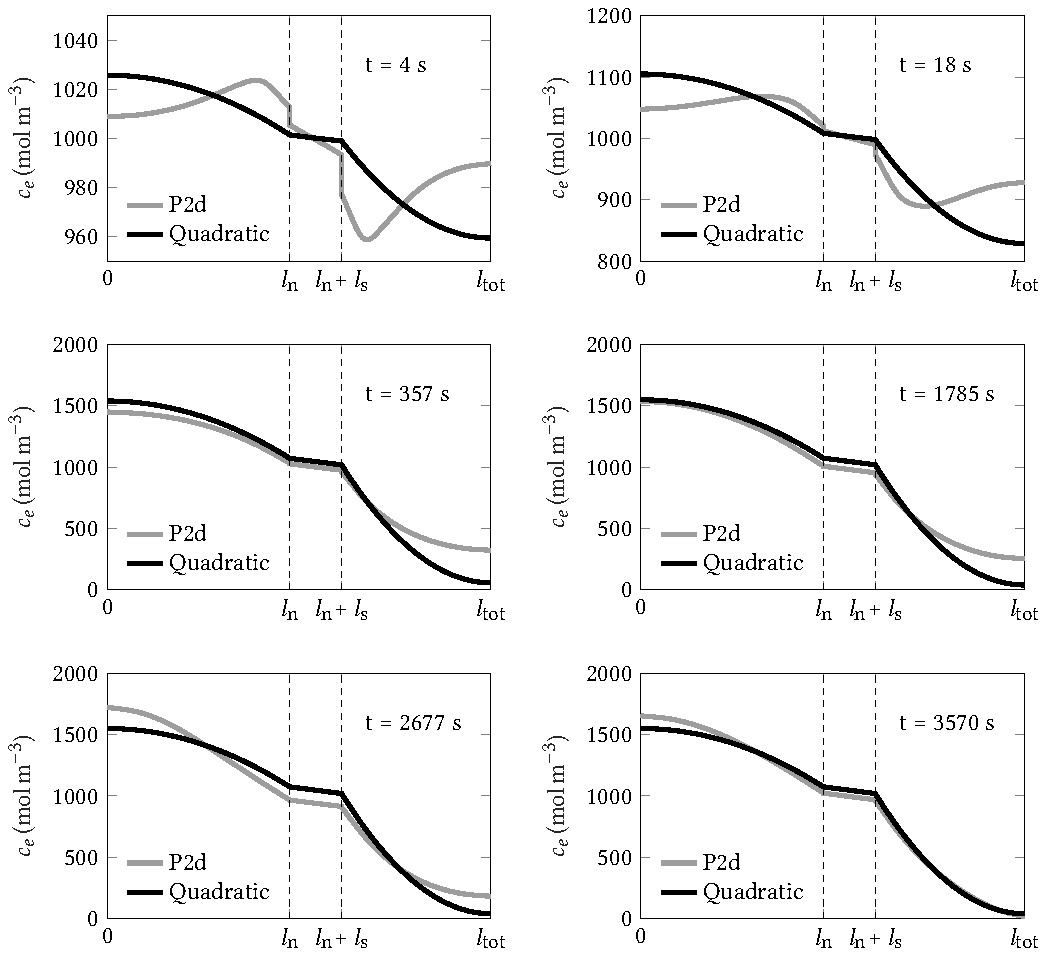
\includegraphics[width=\textwidth]{4/figures/quadratic_ce_approx_spatial_1C.pdf}
    \caption[Spatial distribution of electrolyte concentration for 1C
    discharge]{Spatial distribution of ionic concentration in electrolyte along
        cell thickness at various snapshots of time for a 1C discharge. The
        concentration profile obtained from simulating the \glsfmtshort{p2d}
        model is used as the reference. The performance of the quadratic model
        is quite poor during the initial transient duration, but improves over
    time as a quasi-steady state is reached.}
    \label{fig:spatialionicconc1C}
\end{figure}


\subsubsection*{Simulation results}
\Cref{fig:spatialionicconc1C} shows  the spatial distribution of  \ch{Li^+} ions
in electrolyte  along the  thickness of  the cell at  various snapshots  of time
obtained by simulation  of the \gls{p2d} and the  quadratic approximation models
using a  1C discharge current. The  \gls{p2d} model's response is  considered as
the reference benchmark.  During the initial transient  phase, the concentration
profile within each electrode region exhibits a characteristic inflection point.
During this phase,  the concentration profile computed by  the parabolic profile
exhibits  a  large deviation  in  terms  of  percentage  error at  each  spatial
location. However, with the passage of time, as a \gls{qss} is established, this
inflection point flattens out, and the quadratic approximation becomes closer to
the  true  concentration value  at  each  spatial  location. Similar  trends  in
behaviour is  exhibited for discharge and  charging at higher C-rates  and these
results are  therefore omitted here  in the  interest of keeping  the discussion
succinct.

It  is important  to  note that  while having  a  spatial concentration  profile
is  useful,  as  seen  in~\cref{eq:electrolytepdwithce}, it  is  the  values  of
concentration  at   the  \emph{current  collector  interfaces}   that  are  most
influential in  computation of the  electrolyte overpotential and hence,  in the
voltage accuracy of the enhanced \gls{spm}. Thus, it is important to obtain this
alternative perspective  of time-evolution  of the electrolyte  concentration at
the two current collectors.

\begin{figure}[!htb]
    \centering
    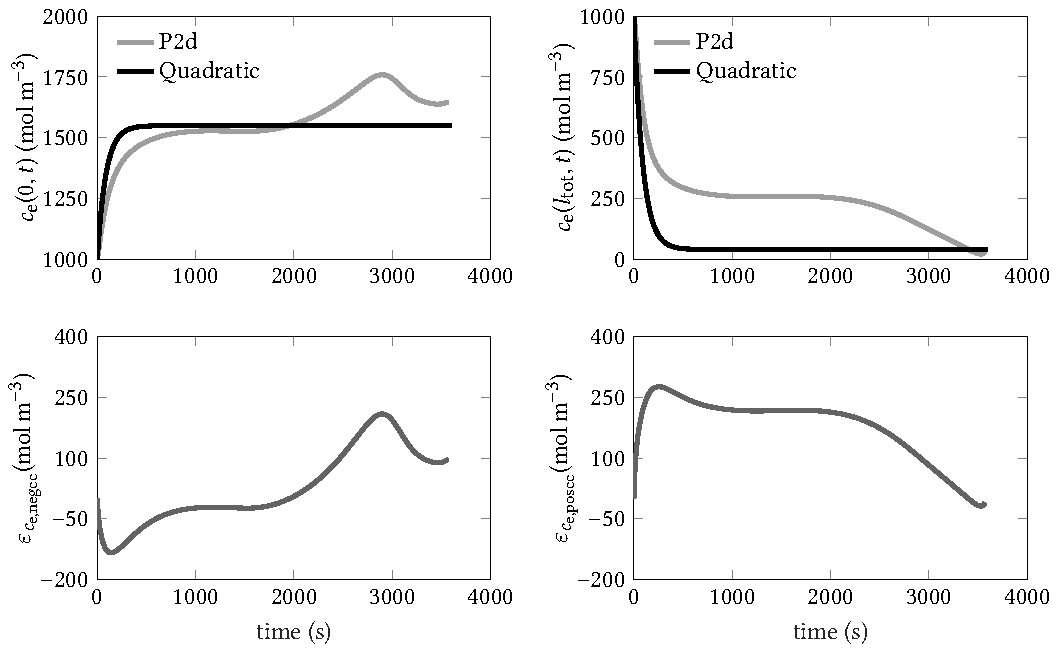
\includegraphics[width=\textwidth]{4/figures/ce_at_cc_1Cdischg.pdf}
    \caption[Ionic concentrations at current collector
    interfaces over time for 1C discharge]{Evolution of ionic concentration over
        time at the two current collector interfaces for a 1C discharge (top
        row). The time evolution of the corresponding error variables is also
    shown (bottom row).}
    \label{fig:temporalcequadratic}
\end{figure}

\Cref{fig:temporalcequadratic} shows  the time evolution of  ionic concentration
in  the electrolyte  at the  two current  collector interfaces  computed by  the
\gls{p2d} and  quadratic approximation  models for a  1C discharge  current. The
concentration  values computed  by  the  \gls{p2d} model  is  considered as  the
reference benchmark. At the negative electrode--current collector interface, the
ionic  concentration  exhibits  a  few oscillations  of  small  amplitude  owing
to  the complex  interactions  of  the ionic  phase  with  the porous  electrode
and  the charge  transfer process  at the  electrode-electrolyte interface.  The
concentration  evolution  predicted  by  the quadratic  approximation  model  is
rather  simplistic  and  is  unable to  capture  this  intricate  time-evolution
pattern.  This  is because  the  governing  equation predicting  time  evolution
of  concentration  in  the  quadratic  approximation  model  is  that  given  by
the  \emph{first-order}  \gls{ode} of~\cref{eq:negliionmolesquadratic}  (with  a
proportional mapping from $Q_\text{e,n}$ to $c_\text{e}(0,t)$). Following system
theory, the step response  of a first order \gls{ode} is  that of an exponential
rise to a final settling value, which  is exactly the shape seen in the top-left
plot of~\cref{fig:temporalcequadratic}.

The ionic  concentration evolution  at the positive  current collector  does not
exhibit major oscillations  and even has a subtle monotonicity  to its response.
However,  the  classical  first  order  response  predicated  by  the  quadratic
approximation model falls short of representing its complete dynamics. Errors of
similar  magnitude  are present  in  the  ionic  concentration at  both  current
collector  interfaces, with  a maximum  absolute error  of \approx\SI{250}{\mole
\per \meter  \cubed}. Similar trends occur  in charging, with a  swapping of the
response pattern of the behaviour at negative and positive electrode interfaces.

\subsubsection*{Analysis and issue of equation deficiency}
In  the author's  analysis  of  the quadratic  approximation  model, the  origin
and  nature  of  its  sub-optimal  performance  can  be  explained  as  per  the
following  rationale.   The  quadratic  approximation  model   uses  a  top-down
approach wherein  the model structure  is pre-assumed  and then the  physics are
made  to  fit within  this  framework.  Given  that  the bottom-up  approach  to
electrolyte  modelling, \ie{}  accounting for  all physical  phenomena and  then
simplifying  them yields  mathematically intractable  and overly  complex models
(see~\cref{sec:electrolyteinclusion} for  a detailed discussion),  this approach
seems to be a pragmatic alternative  to enhancing the \gls{spm} with electrolyte
dynamics.

The  question then  boils  down  to whether  quadratic  approximation is  indeed
the  \emph{best} model  structure  that  can be  assumed  a  priori. The  author
embarked  on a  journey to  find suitable  alternate model  structures, \ie{}  a
single  family of  curves that  will capture  both the  transient and  \gls{qss}
behaviour exhibited by  the ionic concentration. The  open-source MATLAB toolbox
GPTIPS2~\cite{Searson2015}  uses the  state-of-the-art  \gls{mggp} approach  for
symbolic data  mining and is ideally  suited for such symbolic  regression tasks
(fitting a  mathematical equation structure,  and not merely  obtaining best-fit
coefficients to a  pre-assumed curve as in classical numerical  regression, to a
given data).

It  is  important  to  recognize  that  the  key  criteria  that  restricts  the
choice  of gene  sequence  depth as  well  as  the choice  in  number of  parent
mutations  is  the  total  number  of  unknown  symbolic  coefficients  required
to  be   solved  in  the  assumed   model  structure.  There  are   a  total  of
\emph{seven} linear equations available from  the physics of the \gls{dfn} model
(see~\crefrange{eq:cecontinuitynegsep}{eq:Qepbyintegration}).  Thus the  assumed
family  of curves  \emph{cannot}  consist  of more  than  seven coefficients  to
guarantee a  unique solution. Yet  another restriction  on the choice  of curves
arises due to the fact that the behaviour of ionic concentration in the negative
and positive electrode  regions are similar in complexity, and  hence need to be
mathematically described by an identical family of curves.

Upon a close inspection of the  spatial concentration profile from the \gls{p2d}
simulation  results shown  in~\cref{fig:spatialionicconc1C}, it  is evident  the
electrolyte approximation  functions within the  electrode regions is  of higher
complexity than  the approximation  function suitable for  use in  the separator
region. Based on the  results of the quadratic model, it is  clear that at least
two coefficients  are required within the  electrode regions, $n_{\text{c,elec}}
\ge  2$.  There  exists  an  inhibiting  factor  that  prevents  the  use  of  a
lower  order  function within  the  separator.  As  per the  simulation  results
of  the  \gls{p2d}  model,  the  time-domain  change  of  number  of  moles  per
square  meter  in  the  separator   is  non-zero.  Therefore,  a  simple  linear
approximation is immediately  ruled out as per~\cref{eq:sepliionmolesquadratic}.
Among non-polynomial mathematical curves tried (trigonometric, hyperbolic, power
series  among  others),  none  could  obtain  the  relatively  simple  shape  of
the  separator function,  without  reducing  the contribution  from  one of  the
coefficients  to below  machine  precision.  This forces  the  retention of  the
quadratic approximation  function used thus  far (with no missing  terms), \ie{}
$n_\text{c,sep}  = 3$.  Thus, the  overall number  of coefficients  in the  best
possible approximation shall be $2  n_\text{c,elec} + n_\text{c,sep} = 2\cdot2 +
3 = 7$,  which is the total number of  electrolyte-specific physical constraints
available from the \gls{dfn} model. Thus, it can be concluded that the quadratic
approximation model does indeed make the \emph{best} use of all of the available
physical  equations.  The  final  question  remains to  answer  is,  with  these
coefficient limitations, is the quadratic  equation structure indeed the optimal
one. This was investigated through the \gls{mggp} approach.

The GPTIPS2  toolbox uses a variety  of heuristic algorithms from  the theory of
\gls{mggp} to fit a  suitable equation structure for the data  to be fitted. The
dataset  consisted  of the  simulation  results  from  the \gls{p2d}  model,  in
particular  the  values of  electrolyte  concentration  at the  three  different
cell  regions,  captured  at  various  snapshots of  time.  Both  transient  and
\gls{qss}  output  were  fed  into  this symbolic  data  mining  process  and  a
single all-encompassing  family of curves  capable of capturing  the electrolyte
concentration  behaviour  was  sought  for.  However,  with  the  aforementioned
constraints in the number of coefficients results in restriction of the depth of
gene mutations as  well as the number of unconnected  seed populations. The best
equation  set (without  hard constraints,  yet  minimizing the  distance to  the
constraint vector) that the symbolic regression approach yielded was
\begin{alignat}{2}
    c_\ensub(z,t) & = a_2(t) \cosh z^2 + a_1(t) \sinh z + a_0(t) \qquad &  & 0 \le z \le l_\text{n}   \\
    c_\essub(z,t) & = a_5(t) z^2 + a_4(t) z + a_3(t) \qquad &  & 0 \le z \le l_\text{s}   \\
    c_\epsub(z,t) & = a_8(t) \cosh z^2 + a_7(t) \sinh z + a_6(t) \qquad &  & 0 \le z \le l_\text{p}
\end{alignat}
which  although  fits  the  transient  and  \gls{qss}  profiles  well,  violates
the  constraint on  the  number of  coefficients available,  and  results in  an
underdetermined  system  of equations.  Both  the  least-squares and  least-norm
solution of this  system were tried. However, the results  were inferior to that
produced by the baseline quadratic approximation method.

An  attempt  was  made  to  obtain different  mathematical  structures  for  the
transient phase and  \gls{qss} phase. The symbolic regression  output for this
approach are shown in~\cref{tbl:symbreg}.
% -*- root: ../main.tex -*-
%!TEX root = ../main.tex
% this file is called up by main.tex
% content in this file will be fed into the main document
% vim:nospell textwidth=180 foldlevelstart=3 foldlevel=3 conceallevel=0

\begin{table}[!htb]
    \centering
    \caption[Transient \& \glsfmtshort{qss} expressions for electrolyte
    concentration obtained by \glsfmtshort{mggp}]{Best fit expressions for the
        transient and \glsfmtlong{qss} approximaton functions for the
    electrolyte functions obtained by the \gls{mggp} approach}
    \label{tbl:symbreg}
    \begingroup
    \addtolength{\jot}{0.25em}
    \begin{tabular}{@{} c c r @{}}
        \toprule
        \multicolumn{1}{l}{Transient Function} & \multicolumn{1}{c}{\glsfmtlong{qss} Function} & \multicolumn{1}{c}{Region} \\
        \midrule
        $\begin{aligned}
            c_{\text{e,n}_\text{trans}} &= a_1 z^6 \ln z^6 + a_0 \\
            c_{\text{e,s}_\text{trans}} &= a_4 z^2 + a_3 z + a_2 \\
            c_{\text{e,p}_\text{trans}} &= a_6 z^6 \ln z^6 + a_5 \\
        \end{aligned}$ &
        $\begin{aligned}
            c_{\text{e,n}_\text{QSS}} &= a_1 \sinh z^2 + a_0 \\
            c_{\text{e,s}_\text{QSS}} &= a_4 z^2 + a_3 z + a_2 \\
            c_{\text{e,p}_\text{QSS}} &= a_6 \sinh z^2 + a_5
        \end{aligned}$ &
        $\begin{aligned}
            &0 \le z \le l_\text{n} \\
            &0 \le z \le l_\text{s} \\
            &0 \le z \le l_\text{p}
        \end{aligned}$
        \\
        \bottomrule
    \end{tabular}
    \endgroup
\end{table}




Overall, the long and arduous process of symbolic regression was not a success
in this context mainly due to the aforementioned limitations. Perhaps if another
physics-based model alternative to the widely prevalent \gls{dfn} model can be
used as the baseline, more physical governing equations could perhaps be
established, leading to a less restrictive gene-set for coefficient
determination. In summary, the \gls{mggp} symbolic data mining could not
determine a single family of equations that together





